% ----------------------------------------------------
% Literature Review
% ----------------------------------------------------
\documentclass[class=report,11pt,crop=false]{standalone}
% Page geometry
\usepackage[a4paper,margin=20mm,top=25mm,bottom=25mm]{geometry}

% Font choice
\usepackage{lmodern}

% \usepackage{lipsum}

% Use IEEE bibliography style
\bibliographystyle{IEEEtran}

% Line spacing
\usepackage{setspace}
\setstretch{1.20}

% Ensure UTF8 encoding
\usepackage[utf8]{inputenc}

% Language standard (not too important)
\usepackage[english]{babel}

% Skip a line in between paragraphs
\usepackage{parskip}

% For the creation of dummy text
\usepackage{blindtext}

% Math
\usepackage{amsmath}

% Header & Footer stuff
\usepackage{fancyhdr}
\pagestyle{fancy}
\fancyhead{}
\fancyhead[R]{\nouppercase{\rightmark}}
\fancyfoot{}
\fancyfoot[C]{\thepage}
\renewcommand{\headrulewidth}{0.0pt}
\renewcommand{\footrulewidth}{0.0pt}
\setlength{\headheight}{13.6pt}

% Epigraphs
\usepackage{epigraph}
\setlength\epigraphrule{0pt}
\setlength{\epigraphwidth}{0.65\textwidth}

% Colour
\usepackage{color}
\usepackage[usenames,dvipsnames]{xcolor}

% Hyperlinks & References
\usepackage{hyperref}
\definecolor{linkColour}{RGB}{77,71,179}
\hypersetup{
    colorlinks=true,
    linkcolor=linkColour,
    filecolor=linkColour,
    urlcolor=linkColour,
    citecolor=linkColour,
}
\urlstyle{same}

% Automatically correct front-side quotes
\usepackage[autostyle=false, style=ukenglish]{csquotes}
\MakeOuterQuote{"}

% Graphics
\usepackage{graphicx}
\graphicspath{{Images/}{../Images/}}
\usepackage{makecell}
\usepackage{transparent}

% SI units
\usepackage{siunitx}

% Microtype goodness
\usepackage{microtype}

% Listings
\usepackage[T1]{fontenc}
\usepackage{listings}
\usepackage[scaled=0.8]{DejaVuSansMono}

% Custom colours for listings
\definecolor{backgroundColour}{RGB}{250,250,250}
\definecolor{commentColour}{RGB}{73, 175, 102}
\definecolor{identifierColour}{RGB}{196, 19, 66}
\definecolor{stringColour}{RGB}{252, 156, 30}
\definecolor{keywordColour}{RGB}{50, 38, 224}
\definecolor{lineNumbersColour}{RGB}{127,127,127}
\lstset{
  language=Matlab,
  captionpos=b,
  aboveskip=15pt,belowskip=10pt,
  backgroundcolor=\color{backgroundColour},
  basicstyle=\ttfamily,%\footnotesize,        % the size of the fonts that are used for the code
  breakatwhitespace=false,         % sets if automatic breaks should only happen at whitespace
  breaklines=true,                 % sets automatic line breaking
  postbreak=\mbox{\textcolor{red}{$\hookrightarrow$}\space},
  commentstyle=\color{commentColour},    % comment style
  identifierstyle=\color{identifierColour},
  stringstyle=\color{stringColour},
   keywordstyle=\color{keywordColour},       % keyword style
  %escapeinside={\%*}{*)},          % if you want to add LaTeX within your code
  extendedchars=true,              % lets you use non-ASCII characters; for 8-bits encodings only, does not work with UTF-8
  frame=single,	                   % adds a frame around the code
  keepspaces=true,                 % keeps spaces in text, useful for keeping indentation of code (possibly needs columns=flexible)
  morekeywords={*,...},            % if you want to add more keywords to the set
  numbers=left,                    % where to put the line-numbers; possible values are (none, left, right)
  numbersep=5pt,                   % how far the line-numbers are from the code
  numberstyle=\tiny\color{lineNumbersColour}, % the style that is used for the line-numbers
  rulecolor=\color{black},         % if not set, the frame-color may be changed on line-breaks within not-black text (e.g. comments (green here))
  showspaces=false,                % show spaces everywhere adding particular underscores; it overrides 'showstringspaces'
  showstringspaces=false,          % underline spaces within strings only
  showtabs=false,                  % show tabs within strings adding particular underscores
  stepnumber=1,                    % the step between two line-numbers. If it's 1, each line will be numbered
  tabsize=2,	                   % sets default tabsize to 2 spaces
  %title=\lstname                   % show the filename of files included with \lstinputlisting; also try caption instead of title
}

% Caption stuff
\usepackage[hypcap=true, justification=centering]{caption}
\usepackage{subcaption}

% Glossary package
% \usepackage[acronym]{glossaries}
\usepackage{glossaries-extra}
\setabbreviationstyle[acronym]{long-short}

% For Proofs & Theorems
\usepackage{amsthm}

% Maths symbols
\usepackage{amssymb}
\usepackage{mathrsfs}
\usepackage{mathtools}

% For algorithms
\usepackage[]{algorithm2e}

% Spacing stuff
\setlength{\abovecaptionskip}{5pt plus 3pt minus 2pt}
\setlength{\belowcaptionskip}{5pt plus 3pt minus 2pt}
\setlength{\textfloatsep}{10pt plus 3pt minus 2pt}
\setlength{\intextsep}{15pt plus 3pt minus 2pt}

% For aligning footnotes at bottom of page, instead of hugging text
\usepackage[bottom]{footmisc}

% Add LoF, Bib, etc. to ToC
\usepackage[nottoc]{tocbibind}

% SI
\usepackage{siunitx}

% For removing some whitespace in Chapter headings etc
\usepackage{etoolbox}
\makeatletter
\patchcmd{\@makechapterhead}{\vspace*{50\p@}}{\vspace*{-10pt}}{}{}%
\patchcmd{\@makeschapterhead}{\vspace*{50\p@}}{\vspace*{-10pt}}{}{}%
\makeatother

% Tables
\usepackage{multirow}
\usepackage{longtable}
\usepackage{tabularx}
\makenoidxglossaries

\newacronym{radar}{RADAR}{Radio Detection and Ranging}
\begin{document}
\ifstandalone
\tableofcontents
\fi
% ----------------------------------------------------
\chapter{ Mechanical Casing and Housing (MRBMAT004)\label{ch:literature}}
% \epigraph{}%
    % {\emph{---Carl Sagan}}
% \vspace{0.5cm}
% ----------------------------------------------------

% Before we even start on the first point, we should have a brief intro to talk about what it is we are doing. 
% Before this in chapter 1 will be our problem statement. 
% This is what I suggest: This literature delves into previous research articles pertaining to wildlife monitoring and related fields to better understand the approach that needs to be taken to design an effective camera module. This review will look into existing solutions (both the successes and failures). Data acquisition methods were also investigated. Integration of camera traps with IoT, sensing and power supply requirements were researched as well as looking into camera traps being situated in an urban setting with the risk of theft or damage from weather conditions. 
%Chapter 
%Mechanical Casing and Housing
\section{Introduction}
This section covers the mechanical case designs crafted for the the remote surveillance system deployed at the the Starlings’ nests located within the University of Cape Town for Sally who works at the Fitz Patrick Institute. The goal for this project was enhance nest surveillance through innovative technological solutions. These enclosures serve as the protective shell for our electronic components, safeguarding them against the elements while ensuring optimal functionality. By providing robust protection against environmental factors such as moisture, dust, and temperature fluctuations, the mechanical cases play a crucial role in the reliability and longevity of the surveillance system.
\newline

The surveillance system addresses existing challenges and gaps in current methods of monitoring bird nests by providing real-time data collection, minimizing disturbance to nesting birds, and enabling remote observation capabilities. Traditional nest monitoring methods often rely on manual observation, which can be time-consuming, labour-intensive, and disruptive to nesting birds. Our system offers a non-invasive alternative that allows researchers to gather valuable data without causing undue stress to the bird population.
\newline

The mechanical cases discussed in this section will house the Transmitter and Receiver circuitry systems that aim to solve the surveillance of the nests. This section discusses the design decisions, material choices and processes undertaken to realise the ‘final’ prototype. 
A comprehensive breakdown of the design processes, material choices, and iteration phases involved in the development of the mechanical cases. Exploring the intricacies of each design iteration, discussing the rationale behind design decisions and the challenges encountered during the prototyping process. Additionally, results for, testing and evaluation efforts, offering insights into the performance and effectiveness of the 'final' prototype. Finally, we will draw conclusions based on our findings and discuss potential avenues for future research and development in the field of avian monitoring technology.
\newline

\subsection{Requirements, Specifications, and Acceptable Prototype}
•	Size: 6x6x8cm\newline
•	Receiver case: handheld capability or mounting option\newline
•	Transmitter and receiver cases: safely house the sensor and power module circuits.\newline
•	Circuit protection from environmental conditions and theft prevention. \newline
•	Ease of access for maintenance and user experience.\newline
•	Compatibility with monitoring equipment.\newline
\newline

\section{Design Process}
\subsection{First Iteration Prototype}
The first iteration of the prototype was a simple rectangular box. During the initial stages of the design process, there was limited scope and clarity regarding the project requirements, prompting the development of a basic prototype to initiate discussions with stakeholders.
\newline

However, upon further refinement of the project specifications, it became evident that the initial rectangular design did not align with Sally's requirements, particularly in terms of size. The dimensions of the prototype were arbitrary and did not meet the specified 6x6x8cm dimensions. This discrepancy highlighted the need for clearer communication and adherence to design specifications from the outset of the project.
\newline

Additionally, the choice of PLA material for the prototype was based on availability, without consideration of alternative materials such as PETG, which offers superior properties for this application. The transition to PETG, as suggested by Ryan Jones, was later explored to address concerns related to material durability and performance.
\newline

One notable feature of the first iteration was the inclusion of a sliding mechanism for the open/close function. While this mechanism provided ease of access to the internal components, it posed challenges in terms of sealing effectiveness against moisture, dust, and water ingress. This limitation underscored the importance of robust sealing methods to ensure environmental protection and longevity of the electronic components housed within the enclosure.
\newline

Furthermore, the rectangular shape of the prototype presented challenges in airflow management, potentially leading to airflow turbulence or restrictions within the enclosure. While passive cooling solutions could be employed, such as ventilation holes, the design lacked provisions for active cooling mechanisms, which may be necessary to maintain optimal operating temperatures for sensitive electronics.
\newline

Despite these limitations, the rectangular design demonstrated efficiency in space utilization, offering maximum volume for component placement and organization. Moreover, its geometric simplicity facilitated ease of fabrication, reducing manufacturing complexity and costs associated with more intricate shapes.
\newline

Overall, the first iteration prototype served as a valuable learning experience, highlighting the importance of clear requirements definition, material selection, sealing methods, and considerations for airflow management in the design process. These insights informed subsequent iterations towards the development of a more refined and functional final prototype.
\newline

\subsection{Second Iteration}
The second iteration resembled a pitched roof house. This design idea was perfect until the size constraints were brought forth. Secondly, the pitched roof also limits and reduces the size of the already small dimensions of the specifications given by Sally: 6x6x8cm. 
\newline
This design had ventilation holes and forced cooling using a fan was considered. This fan would require a timer and trigger signal. This design had better airflow management as it promoted natural convection through the ventilation peaks at the peak without the need for additional cooling. The pitched roof enclosures blend seamlessly into outdoor environments, providing camouflage and enhancing the overall aesthetic appeal. However, concerns arose regarding the practicality of this design, particularly regarding size constraints and the need for additional cooling mechanisms as a fan would put added strain on the power supply and increase power losses.
\newline

\subsection{Material used}
% https://all3dp.com/2/plavsabsvspetgdifferencescompared/#google_vignette  
PLA, ABS and PETG are the most popular and readily available filaments out there. However, they are not equally suitable for every printing job as they have different qualities.
\newline

\subsubsection{PLA (Polylactic Acid)}
PLA is a widely used 3D printing material known for its ease of printing and low cost. Derived from renewable sources like corn starch, PLA is considered environmentally friendly, although it is more accurately described as industrially compostable rather than biodegradable. Its benefits include easy printing with no clogging issues, low print temperature, and affordability. However, PLA tends to deform or melt in high heat, making it unsuitable for heat resistant applications. It is also brittle and less sturdy compared to materials like ABS or PETG, making it better suited for aesthetic uses rather than mechanical ones.
\newline

\subsubsection{ABS (Acrylonitrile butadiene styrene)}
ABS (Acrylonitrile Butadiene Styrene) is a durable thermoplastic commonly used in 3D printing, injection molding, and machining. While it offers increased durability and resistance to water compared to PLA, it can emit unpleasant fumes during printing. ABS is known for its strength, toughness, and heat resistance, making it suitable for everyday items. However, it may degrade over time when exposed to prolonged moisture, and it is prone to dust accumulation. Despite its drawbacks, ABS can be easily finished post printing using acetone, making it suitable for aesthetic prints.
\newline

\subsubsection{PETG (Polyethylene terephthalate glycol)}
PETG is a popular choice for applications requiring food safety due to its excellent material properties. While it offers superior water resistance compared to PLA and ABS, printing PETG can be challenging due to its tendency to string during printing. PETG is known for its durability, impact resistance, and UV resistance, making it suitable for outdoor applications. However, it is prone to scratching and requires high printing temperatures, which contribute to stringing issues. Overall, PETG is widely regarded as a food safe filament with excellent mechanical properties.
\newline

Comparisons
\begin{table}[h]
\centering
\begin{tabular}{|>{\raggedright\arraybackslash}p{0.25\linewidth}|>{\raggedright\arraybackslash}p{0.25\linewidth}|>{\raggedright\arraybackslash}p{0.25\linewidth}|>{\raggedright\arraybackslash}p{0.25\linewidth}|}
\hline
 & \textbf{PLA} & \textbf{ABS} & \textbf{PETG} \\ \hline
Temperature & 180-220°C & 210-250°C & 220-250°C \\ \hline
Heated Bed Required & No & 210-250°C & 220-250°C \\ \hline
Enclosure & Does not require an enclosure & ABS is quite susceptible to drafts. Would benefit from an enclosure, to prevent warping and cracking & Does not require an enclosure \\ \hline
Post Processing & Filling, sanding, and priming are the primary methods. There are no safe chemical agents. & Easy to smooth out ABS using acetone & Ethyl acetate can be used to smooth PETG. Filling, sanding, and priming also work \\ \hline
Strength and Durability & Low-to-medium strength filament given its low heat and chemical resistance. & Medium-to-high strength filament, as it will sooner bend than break and has a higher impact, heat, and chemical resistance than PLA. & Medium-to-high strength filament. Mostly like ABS but is superior in strength \\ \hline

\end{tabular}
\end{table}


\begin{table}
    \centering
    \begin{tabular}{|>{\centering\arraybackslash}p{0.25\linewidth}|>{\centering\arraybackslash}p{0.25\linewidth}|>{\centering\arraybackslash}p{0.25\linewidth}|>{\centering\arraybackslash}p{0.25\linewidth}|} \hline 
Toxicity and Odour & Low odour and no toxicity & Has considerable odour and toxicity. & No odour or toxicity \\ \hline
Best Use Cases & Applications that do not have any specific functional requirements. & Often used in functional items that are used frequently or need to be durable. E.g. Drone frame & Excellent for items in contact with food and UV exposure, great for functional parts \\ \hline
    \end{tabular}
    \caption{Caption}
    \label{tab:my_label}
\end{table}

\subsection{Dual and Single enclosure considerations}
In evaluating enclosure design options, a thorough analysis reveals the nuanced advantages of single and dual enclosure configurations. Single enclosures offer notable benefits such as efficient space utilization, simplified installation procedures, streamlined maintenance workflows, and potential cost savings due to component consolidation. However, they also pose challenges in thermal management, necessitating meticulous attention to airflow dynamics and heat dissipation strategies. Furthermore, comprehensive dustproofing measures are imperative to mitigate the risk of contamination and ensure long-term reliability.
\newline

Conversely, dual enclosure setups introduce unique advantages that contribute to the overall resilience and adaptability of the surveillance system. The modular nature of dual enclosures facilitates enhanced system flexibility, allowing for seamless component replacement, upgrades, or reconfigurations without disrupting the entire system. Moreover, the isolation of components within separate enclosures minimizes the risk of interference or contamination, ensuring optimal performance and reliability. The redundancy provided by dual enclosures offers an added layer of security, ensuring continuous operation even in the event of enclosure failure or malfunction.
\newline

Additionally, the customization potential inherent in dual enclosures enables tailored solutions to meet specific application requirements or environmental conditions. From optimized thermal management strategies to tailored dustproofing mechanisms, dual enclosures provide a versatile platform for finetuning system performance and resilience. By segregating components based on thermal characteristics, dual enclosures facilitate more effective heat distribution and dissipation, mitigating the risk of localized overheating and component degradation.
\newline

Furthermore, the independent sealing mechanisms of dual enclosures simplify dustproofing efforts, allowing for targeted measures to prevent dust ingress and contamination. By customizing dust filters and seals for each enclosure, the overall reliability and longevity of the surveillance system are enhanced, ensuring consistent performance even in harsh or dusty environments.

\subsection{Shape Considerations}
Each shape offers unique advantages and disadvantages, influencing space efficiency, aerodynamics, aesthetics, manufacturing complexity, and application-specific requirements.
\newline

Rectangular enclosures excel in efficient space utilization and ease of manufacture, making them suitable for accommodating complex electronic assemblies. However, they may lack optimal aerodynamics and aesthetic appeal compared to other shapes.
\newline

Cylindrical enclosures distribute stress more evenly and offer 360-degree access, making them robust and versatile for various applications. Yet, they may suffer from space inefficiency and manufacturing complexity.
\newline

Tapered or sloped enclosures prioritize improved aerodynamics and aesthetic appeal, optimizing space utilization while posing challenges in design complexity and manufacturing.


\section{Final Design Prototype}
The implementation of two separate electronic enclosure designs for the transmitter and receiver subsections was pivotal in addressing thermal concerns and meeting the distinct requirements of each subsystem. This separation not only improved temperature management but also allowed for increased airflow within each enclosure. Furthermore, considering that the transmitter and receiver subsystems are exposed to different environmental conditions and demand varied parameters for system longevity, this tailored approach ensured optimal performance and durability.
\newline

\subsection{Transmitter Case}
The final design for the mechanical cases for the transmitter subsection was chosen to be a rectangular box, carefully crafted to optimise functionality and environmental protection. It consisted of ventilation holes strategically placed to promote aeration and better airflow management, the design aimed to maintain optimal operating conditions for the enclosed components. Four vents were positioned at the base of the enclosure, each with a 5mm diameter and spaced 30mm apart, allowing air to enter from distinct locations. To prevent ingress of pests, debris, and dust, mesh screen filters covered these vents, while also minimizing the entry of water.
\newline

Four rectangular extrusions, situated 9mm above the base of the box, provided mounting or adhesive points for the Vero boards. This elevated placement reduced contact with any water that might enter through the base vents, ensuring the integrity of the components. Moreover, this design allowed for sufficient space for cool air to circulate around the boards.
\newline

To further enhance thermal management, aluminium heatsinks were strategically placed next to resistive and heat prone components. The orientation of the heatsink fins facing vertically upwards facilitated the natural convection process, whereby warm air rises. This directed the heat away from the components and towards the top of the enclosure. This is because warm air has lower density than cold air hence it rises. 
\newline

Additionally, three vents on either side of the box were incorporated to facilitate the removal of warm air from within the enclosure. This prevented the accumulation of warm air and the formation of a low-pressure cell, ensuring efficient airflow throughout the enclosure.
\newline

To tightly seal the enclosure a lid screw was used to minimise dust and water which was better than the sliding open/close mechanism used before.
\newline
For water and moisture management, a desiccant, silica gel was used to remove or absorb moisture from the electronic enclosure.
\newline

\subsection{Safety mechanisms and waterproof}
Mounting the rectangular enclosure is crucial for both practical functionality and ensuring safety and security. By rigidly attaching the enclosure to a stable structure like a wall or pole, it reduces the risk of unauthorized access to its internal components. This means it is much harder for people without permission to tamper with or steal the system. The act of mounting also acts as a strong deterrent against theft or vandalism, as it makes it clear that the system is secure and not easily removable. Additionally, securely mounting the enclosure ensures it can withstand external forces like wind or impact, making it more durable. It also helps the system comply with safety regulations, ensuring it meets industry standards. Adding features like tamper-resistant mechanisms further enhances security, making it even harder for unauthorized access. Overall, mounting the rectangular enclosure not only serves practical purposes but also plays a vital role in protecting the system and ensuring it functions effectively for a long time.
Mounting the enclosure was deemed a superior safety and security measure, particularly due to the elevated and often remote locations of Starlings' nests, where human access is infrequent. Opting for mounting over traditional locking mechanisms offers a practical solution, ensuring the system's protection without the complexities associated with locks. By rigidly attaching the enclosure to a stable structure, such as a wall or pole, the system's integrity is effectively preserved, mitigating the risk of tampering or theft. This approach not only enhances security but also aligns with the practical constraints of the surveillance environment, where accessibility is limited.


\begin{figure}[H]
    \centering
    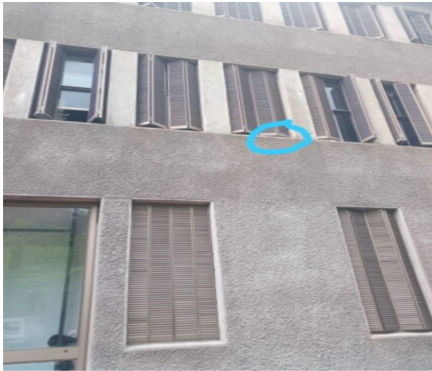
\includegraphics[width=0.5\linewidth]{literature-review/FrontMatter/nest.png}
    \caption{Enter Caption}
    \label{fig:enter-label}
\end{figure}

 
In the ongoing development of the electronic enclosure, a transition has been made from a sliding open/close mechanism to a lid screw configuration. This upgrade aims to provide a more robust closure, effectively minimizing the intrusion of dust and water, while also enhancing security for the enclosed electronics.
\newline

Additionally, to address water and moisture management within the enclosure, silica gel desiccant packs have been integrated into the design. These packs serve as an effective solution for moisture absorption, ensuring the internal environment remains dry and conducive to the optimal functioning of the electronic components. Furthermore, the potential addition of cotton alongside the silica gel desiccant packs can provide an extra layer of moisture protection, especially in environments with high humidity levels or where condensation may occur. Cotton's ability to absorb excess moisture and function as a buffer between electronic components and desiccant packs offers additional assurance against moisture infiltration.
\newline

\subsubsection{Material of Choice}
PETG was the material of choice for the enclosure. PETG offers UV resistance, ensuring the enclosure's structural integrity and optical clarity under prolonged sunlight exposure. Its weather resistance enables it to withstand extreme temperatures, both cold and hot, without compromising its mechanical properties. PETG's strength and loadbearing capacity make it suitable for housing electronic components securely. Importantly, PETG is nontoxic and does not emit harmful gases, aligning with your sustainability goals. Additionally, its recyclable nature promotes responsible material usage, further enhancing the project's sustainability. 
\newline

There were two enclosures designed for the transmitter subsection housing, one for the power module and the other for the sensing circuitry discussed in the other two sections of the report. The dual enclosure method was implemented based on the advantages discussed above. Moreover, it allowed for modular design for each of the systems’ requirements. 
\newline

The power enclosure had all the design considerations discussed above: a lid screw, four vents at the bottom, three on either side of the box, four extrusions for Veroboard, and lastly four exterior extrusions with holes for mounting.
\newline
\begin{figure}[H]
    \centering
    \includegraphics[width=0.5\linewidth]{image1.png}
    \caption{Enter Caption}
    \label{fig:enter-label}
\end{figure}



%%%add the power house
 
The sensing circuitry housing had the same design as the housing for power and had additional openings for the camera sensor, 5 PIR sensors and the 2 LDRs, so that surveillance can be achieved remotely while the housing is mounted. The housings are to be mounted close to the nests which would be easy given where the nests are on campus. 
 %%add thiyashans hous

\begin{figure}[H]
    \centering
    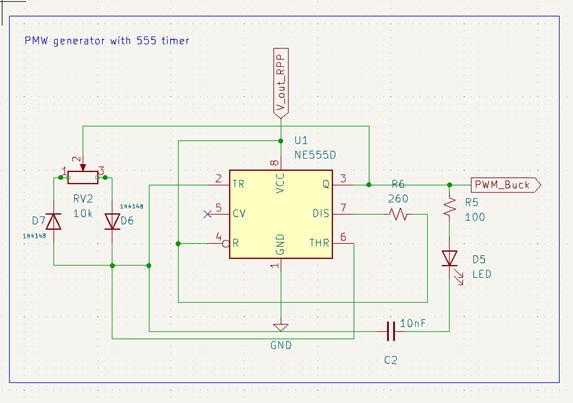
\includegraphics[width=0.5\linewidth]{image.png}
    \caption{Enter Caption}
    \label{fig:enter-label}
\end{figure}

 
\subsection{Receiver Case}
The receiver module material was chosen to be ABS, since it is durable and can be used for consumer daily needs. ABS’ smooth texture and durability and impact resistance made it a suitable material choice for the handheld receiver module.
\newline

The enclosure design included a carefully cutout area to display the LCD output, with a detachable clip side serving as a convenient access point for buttons, eliminating the need for enclosure disassembly. 
\newline

Additionally, a removable latch-sliding mechanism provided port access and simplified battery replacement, as the battery was located on the sliding mechanism side. The generous opening on the sliding mechanism side facilitated effortless battery changes. Prioritizing portability, the enclosure was designed to be handheld, with a compact size ensuring easy readability of LCD display information. This module was bought and had to be assembled and cut the LCD screen part. The removable clip side for the button side made this case attractive as it would be easier to cut holes on the clip or just remove the clip when wanting to access and interface with the buttons. The screw assembled and joined case ensured secure assembly, featuring extrusions for Veroboard placement and a divider allowing for the partitioning of different circuit systems within the enclosure.
\newline

The receiver module did not have specific dimensions but was required to accommodate an 8x4cm LCD area and house the receiver circuitry and its power requirements. This was a single enclosure, and was chosen for the reasons already outlined above, such as efficient space utilization, simplified installation procedures, streamlined maintenance workflows, and potential cost savings. The enclosure design allowed for better airflow, with the removable latch sliding mechanism and LCD cutout contributing to ventilation. Storage conditions were expected to be room temperature, with user requirements limited to handheld, LCD display output and button access, while ensuring circuit integrity and weight support.


 
\begin{figure}[H]
    \centering
    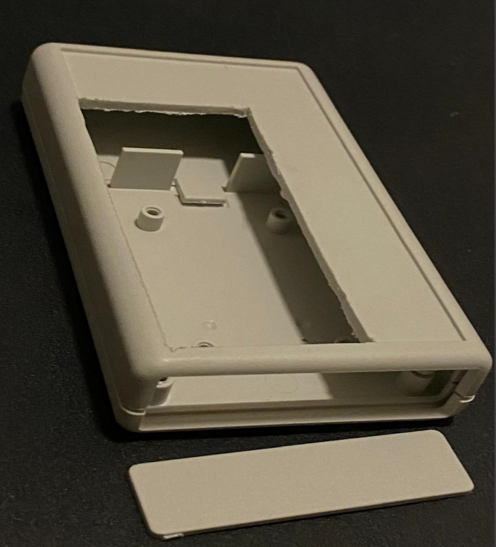
\includegraphics[width=0.5\linewidth]{receiver_house.png}
    \caption{Enter Caption}
    \label{fig:enter-label}
\end{figure}




 

\section{Acceptable Test Procedures}
 
1. Material Durability and Impact Resistance Test:
 Drop tests were conducted from various heights to assess the durability and impact resistance of the ABS and PETG materials. Observations were made for any signs of damage, cracking, or deformation after each drop test. None were found so passed. 
 \newline
 

2. Ventilation and Airflow Test:
    The enclosure designs with ventilation holes and extrusions were 3D printed. Temperature and humidity sensors were used to measure airflow and temperature distribution within the enclosures.
    The effectiveness of the ventilation system in maintaining optimal operating conditions for enclosed components was evaluated.
    \newline

3. Weather Resistance Test:
    The 3D printed enclosures were subjected to temperature and humidity variations in a controlled environment. Exposure to UV light was done by placing the enclosures on the window for days. The enclosures were assessed for any signs of degradation, discoloration, or moisture ingress after exposure. None were found so passed.
    \newline

4. Lid Screw Seal Integrity Test:
    The enclosures were 3D printed with lid screw mechanisms. The lid and housing were mated on SolidWorks to ensure that they fit together through simulation. The lid was screwed to the enclosure as seen in the pictures above.
    \newline
    

5. Moisture Management Test:
 Silica gel desiccant packs and cotton were placed inside the 3D-printed enclosures. Moisture levels inside the enclosures were monitored over time using moisture indicators. The effectiveness of moisture absorption and management by the desiccant packs and cotton was verified.
\newline

6. Portability and Handheld Use Test:
The 3D-printed enclosures were assembled, and the bought design for handheld use was assessed. The comfort and ease of handling were evaluated, ensuring easy access to buttons and readability of the LCD display. Passed.
\newline

7. Assembly and Disassembly Test:
    The 3D-printed enclosures were assembled and disassembled multiple times to assess the ease of assembly and accessibility to internal components. Wear or damage to the enclosure components during assembly and disassembly was checked. Passed
    \newline

8. Mounting and Security Test:
 The 3D printed enclosures were attached to stable structures using mounting brackets or adhesive mounts. Force or pressure was applied to the mounted enclosures to simulate external impacts, verifying their stability and security. Passed. 
 \newline

9. Functionality and Compatibility Test:
Electronic components and power sources were installed inside the 3D printed enclosures. The functionality of the LCD display, buttons, and other components was evaluated to ensure proper operation. Compatibility with the specified electronic components and power requirements was verified.
Failed. The enclosures were scaled down by the Prusa slicer and were not the same dimensions as given on solid works, hence the printed enclosures were small, and the lid had to be cut as it was not scaled to fit the small enclosures. 
\newline


Waterproof: silica gel https://www.ygenclosure.com/article/howtopreventcondensationinyourelectricalenclosures.html






% ----------------------------------------------------
\ifstandalone
\bibliography{../Bibliography/References.bib}
\printnoidxglossary[type=\acronymtype,nonumberlist]
\fi
\end{document}
% ----------------------------------------------------
